\documentclass[12pt]{article}

%%%%%% Packages
\usepackage{amsmath, amssymb}
\usepackage{graphicx}


%%%%%% New commands
% iid text above the distribution sign
\newcommand{\iid}{\overset{\mathrm{\mathrm{iid}}}{\sim}}
% Expectation symbol
\DeclareMathOperator*{\E}{\mathbb{E}}
% Partial differentiation shorthand
\newcommand{\dpart}[2]{\frac{\partial #1}{\partial #2}}


%%%%%% Opening details
\title{Ito Integral}
\author{Treacher}


\begin{document}

\date{}
\maketitle

\begin{abstract}

\noindent Just some notes about the Ito integral, along with some preliminary information about Riemann and Riemann-Stieltjes integration. Summarised from various places online, including but not limited to:
\begin{itemize}
	\item https://www.youtube.com/watch?v=vHn1M6pUAWg
	\item http://www.columbia.edu/~ks20/FE-Notes/4700-07-Notes-Ito.pdf
\end{itemize}

\end{abstract}

\section{Preliminaries}
\subsection{Riemann integration}
For a regular non-stochastic function (black line in figure \ref{fig:riemannSums}), you can use Riemann integration to approximate the integral. This approach involves:
\begin{itemize}
	\item Divide range of integration into set of subintervals $P=\{t_0,t_1,t_2,...,t_n\}$
	\item Over all subintervals, calculate the lower and upper Riemann sums which represent the areas of the rectangles of width equal to the subinterval, and heights equal to the minimum and maximum function value in that interval (see figure \ref{fig:riemannSums}):
	\begin{itemize}
		\item Lower sum: $L = \sum_{i=1}^{n}\mathrm{min}\{f(t_i)\}\cdot(t_i-t_{i-1})$
		\item Upper sum: $U = \sum_{i=1}^{n}\mathrm{max}\{f(t_i)\}\cdot(t_i-t_{i-1})$
	\end{itemize}
	\item For a given function and a small number of partitions, the lower sum will be smaller than the upper sum.
	\item As the number of partitions increases, the values of the two sums will converge toward eachother (if the integral exists).
	\item When the values of the sums intersect, that value is taken to be the Riemann integral of that function over the relevant limits.
\end{itemize}

\begin{figure}[h!]
	\centering
	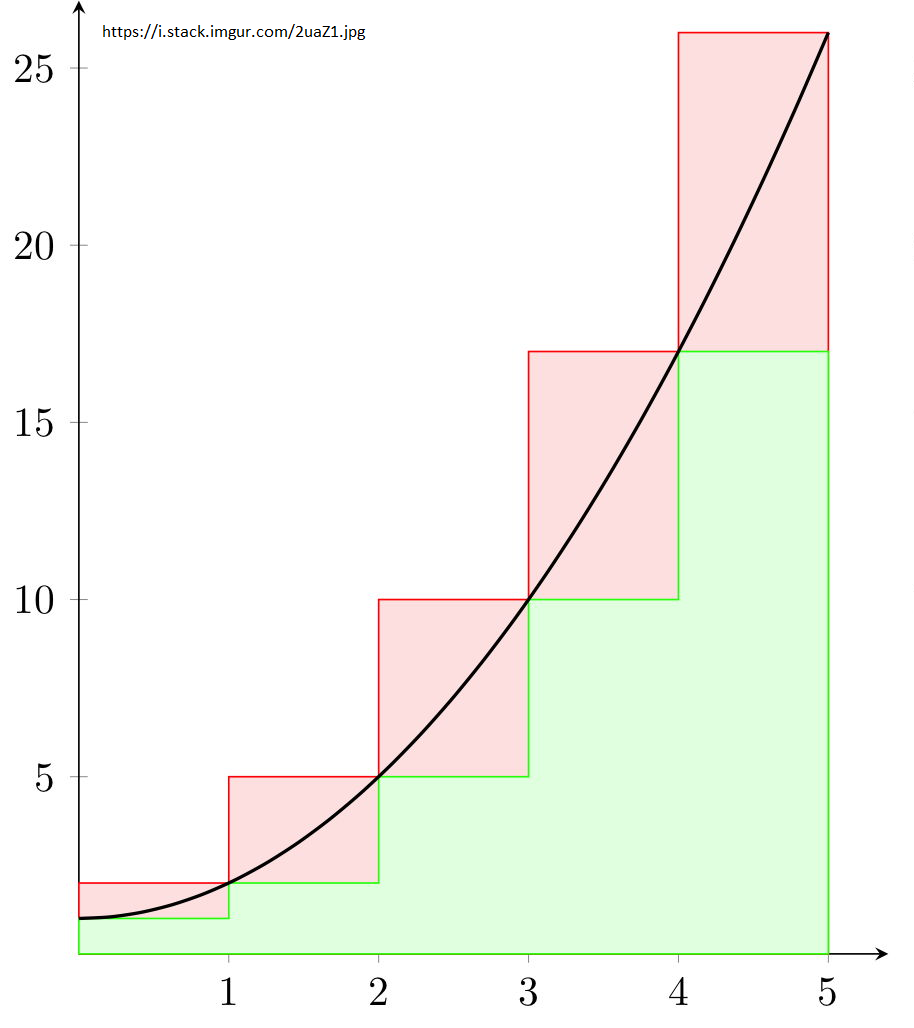
\includegraphics[width=0.8\linewidth]{riemannSums.png}
	\caption{Lower (green) and upper (red) Riemann sums of a function (black)}
	\label{fig:riemannSums}
\end{figure}

\subsection{Riemann-Stieltjes integration}

This is a generalisation of Riemann integration, but where Riemann uses fixed subintervals of $(t_i-t_{i-1})$ as the integrator (d$t$), the Stieltjes approach uses a monotonic function instead.\\
\\
Now the analogous lower and upper sums are:
\begin{eqnarray}
	L &= \sum_{i=1}^{n}\mathrm{min}\{f(t_i)\}\cdot(g(t_i)-g(t_{i-1}))\\
	U &= \sum_{i=1}^{n}\mathrm{max}\{f(t_i)\}\cdot(g(t_i)-g(t_{i-1}))
\end{eqnarray}
\noindent where $g(t_i)>g(t_{i-1})$ when $t_i>t_{i-1}$\\
\\
Imagine a 3D plot of $f(t)$ vs $g(t)$ vs $t$ such as in  figure \ref{fig:stieltjesIntegration}.
\begin{figure}[h!]
	\centering
	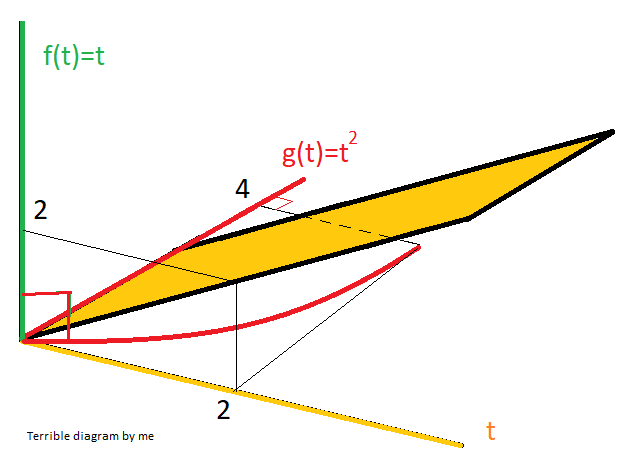
\includegraphics[width=0.8\linewidth]{stieltjesIntegration.png}
	\caption{Stieltjes framework with the integrand $f(t)=t$ and integrator $g(t)=t^2$.}
	\label{fig:stieltjesIntegration}
\end{figure}

\noindent The lower sum will be the value of $f(t=0)=0$ multiplied by the corresponding change in value of $g(t)$. This will be zero. The upper sum will be the max value of $f(t)$ over the range of $[0,2]$ which is $f(2)=2$ multiplied by the change in value of integrator: $g(t_i)-g(t_{i-1})=2^2 - 0^2=4$, giving a final result of 8.\\
\\
Same logic as above applies when increasing the number of partitions until the upper and lower sums intersect, which represents the value of the integral (if it exists). Note that when adding more partitions, the should be placed at equally spaced values of the integrator $g(t)$. In this example with $g(t)=t^2$, the half way point would be half the max value of $g(t)$ which is 4, evaluated at the corresponding value of $t$. This would be $t=\sqrt{2}$.


\section{Brownian motion as integrator}

The above Stieltjes approach doesn't translate to using Brownian motion as the integrator because of its fractal and zig-zagy nature. These factors make proofs of convergence difficult and motivate the choice for a different kind of integration: One using `simple functions'

\section{Definition}

Ito integral is defined as:

\begin{equation} \label{eq:itoIntegral}
	\int_{0}^{t}X_a\,\mathrm{d}B_s\approx\lim\limits_{k\to\infty}\sum_{i=1}^{k}X(t_{i-1})\cdot(B_{t_i}-B_{t_{i-1}})
\end{equation}


\end{document}
